\section{Regressão Logística}
\label{s.logistic_regression}

\subsection{Problemas de duas classes}
\label{ss.twoclass_problem}

Suponha que tenhamos um problema de classificação binária (i.e. um problema de duas classes, $y \in \{0,1\}$). Uma simples ilustração desse problema é dada a seguir:

 \begin{center}
 	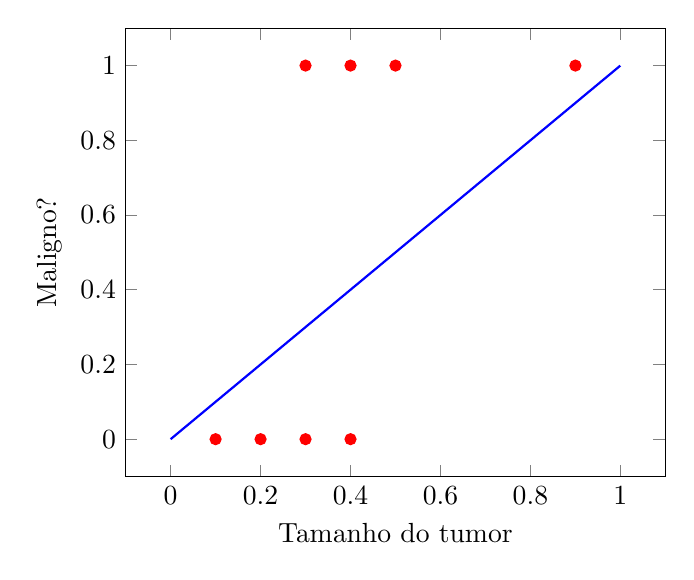
\begin{tikzpicture}[domain=0:1]
  	\begin{axis}[ 
    	xlabel=Tamanho do tumor,
    	ylabel={Maligno?}
  		] 
    	\addplot[blue, thick] {x}; 
    	\addplot[only marks, red] plot coordinates {
        (0.3,1)
        (0.4,1) 
        (0.5,1)
        (0.9,1)
        (0.1,0)
        (0.2,0) 
        (0.3,0)
        (0.4,0)      
    };
  	\end{axis}
	\end{tikzpicture}
 \end{center}
 
Podemos utilizar uma regressão linear aqui, com a seguinte regra:\\se $(h_w(x) > 0.5)$ $y =$ SIM, se não $y =$ NÃO.
 
Entretanto, pode-se ter conjuntos de treinamentos mais complexos. Em tais casos, a Regressão Linear pode não ser plausível para solucionar o problema, como segue:
 
  \begin{center}
 	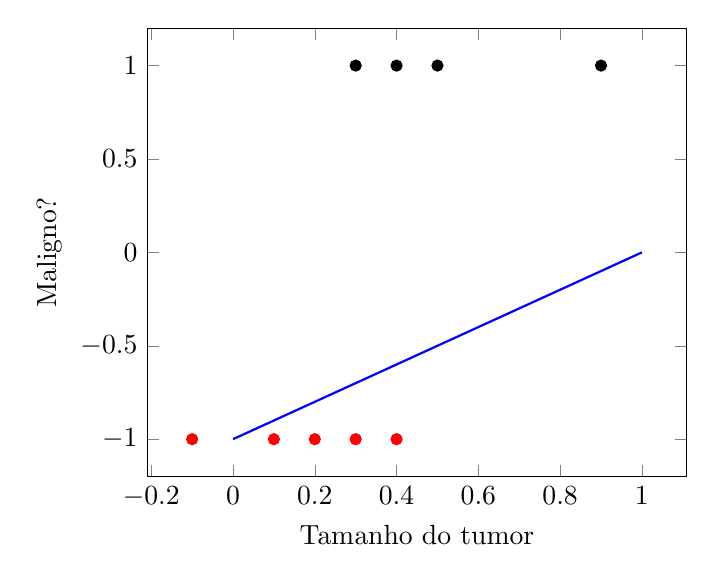
\begin{tikzpicture}[domain=0:1]
  	\begin{axis}[ 
    	xlabel=Tamanho do tumor,
    	ylabel={Maligno?}
  		] 
    	\addplot[blue, thick] {x - 1}; 
    	\addplot[only marks, red] plot coordinates {
        (-0.1,-1)
        (0.1,-1)
        (0.2,-1) 
        (0.3,-1)
        (0.4,-1)      
    };
        \addplot[only marks, black] plot coordinates {
        (0.3,1)
        (0.4,1) 
        (0.5,1)
        (0.9,1)
    };
  	\end{axis}
	\end{tikzpicture}
 \end{center}
 
Portanto, mesmo quando sabemos que a saída de nosso problema é 0 ou 1, é estranho que $h_w(x)$ possa assumir valores $> 1$ ou $< 0$. Tal como, se sabemos que nossa saída está no intervalo $h_w(x) \in [0,1]$, podemos aplicar a \textbf{Regressão Logística} para tal caso. Embora seja chamado de Regressão Logística, ela é uma técnica de \textbf{classificação}.\\
 
\textbf{Modelo da Regressão Logística}\\

\begin{center}
 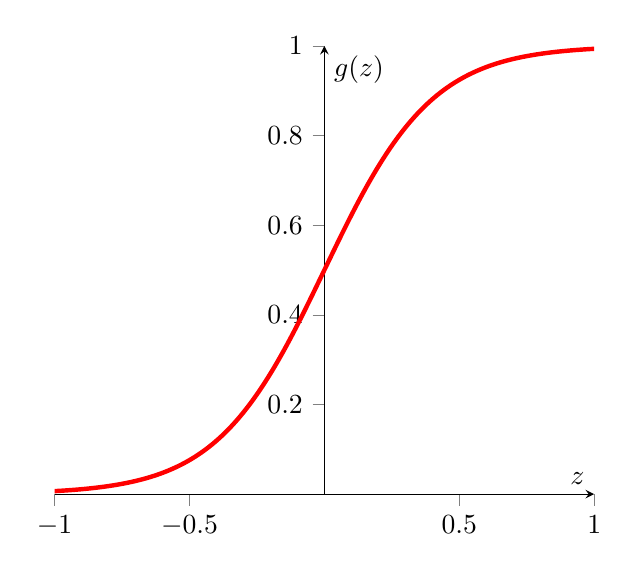
\begin{tikzpicture}
    \begin{axis}[
    	legend pos=north west,
        axis x line=middle,
        axis y line=middle,
        xmin=-1,
        xmax= 1,
        ymin= 0,
        ymax= 1,
        xlabel=$z$,
        ylabel=$g(z)$,
        tick align=outside,
        enlargelimits=false]
      \addplot[domain=-1:1, red, ultra thick,samples=500] {1/(1+exp(-5*x))};
    \end{axis}
 \end{tikzpicture}
\end{center}
 
Queremos $0 \leq h_w(x) \leq 1$, com $h_w(x) = g(w^Tx)$, onde $g(z) = \frac{1}{1 + e^-z}$.
 
Portanto, temos que:

\begin{equation}
h_w(x) = \frac{1}{1 + e^{-w^Tx}}. 	
\end{equation}

Basicamente, a técnica de Regressão Logística tem por objetivo estimar $w$. Podemos interpretar a saída de hipótese como segue:

\begin{equation}
h_w(x) = P(y = 1 \mid x; w),
\end{equation}

onde significa a probabilidade de $y = 1$ dado $x$ parametrizado por $w$.

\begin{center}
 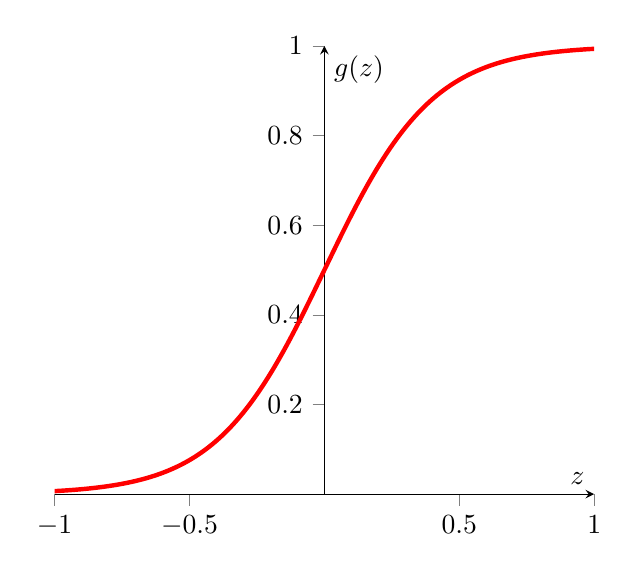
\begin{tikzpicture}
    \begin{axis}[
    	legend pos=north west,
        axis x line=middle,
        axis y line=middle,
        xmin=-1,
        xmax= 1,
        ymin= 0,
        ymax= 1,
        xlabel=$z$,
        ylabel=$g(z)$,
        tick align=outside,
        enlargelimits=false]
      \addplot[domain=-1:1, red, ultra thick,samples=500] {1/(1+exp(-5*x))};
    \end{axis}
 \end{tikzpicture}
\end{center}

\begin{center}
$g(z) \geq 0.5$ quando $z \geq 0$\\
$h_w(x) = g(w^Tx) \geq 0$ quando $w^Tx \geq 0$\\
$h_w(x) = g(w^Tx) < 0$ quando $w^Tx < 0$\\	
\end{center}

Suponha que tenhamos a seguinte situação:

\begin{center}
 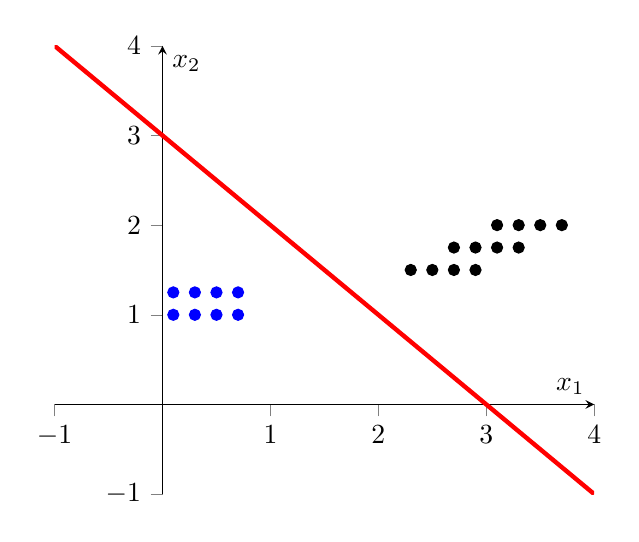
\begin{tikzpicture}
    \begin{axis}[
    	legend pos=north west,
        axis x line=middle,
        axis y line=middle,
        xmin=-1,
        xmax= 4,
        ymin= -1,
        ymax= 4,
        xlabel=$x_1$,
        ylabel=$x_2$,
        tick align=outside,
        enlargelimits=false]
      \addplot[domain=-4:4, red, ultra thick,samples=500] {-x + 3};
      \addplot[only marks, blue] plot coordinates {
        (0.1,1)
        (0.3,1) 
        (0.5,1)
        (0.7,1) 
        (0.1,1.25)
        (0.3,1.25) 
        (0.5,1.25)
        (0.7,1.25)      
    };
        \addplot[only marks, black] plot coordinates {
        (2.9,1.5)
        (2.7,1.5) 
        (2.5,1.5)
        (2.3,1.5)
        (2.9,1.75)
        (2.7,1.75) 
        (3.1,1.75)
        (3.3,1.75)
        (3.7,2)
        (3.5,2) 
        (3.3,2)
        (3.1,2)
    };
    \end{axis}
 \end{tikzpicture}
\end{center}

\begin{center}
$x_1 + x_2 = 3$ (LIMITE DE DECISÃO), corresponde a $h_w(x) = 0.5$\\
$h_w(x) = g(w^Tx) = g(w_0 + w_1x_1 + w_2x_2)$, onde \[W=
  \begin{bmatrix}
    -3 \\
    1 \\
    1 
  \end{bmatrix}\]
\end{center}

Portanto, queremos prever $y = 1$ se $-3 + x_1 + x_2 \geq 0 \Rightarrow x_1 + x_2 \geq 3$.\\

\textcolor{red}{OBS: Falta exemplo do círculo.} \\

Vamos sumarizar o nosso problema:\\

\textbf{conjunto de treinamento:} $X = \{(x_1, y_1), (x_2, y_2), \dots, (x_m, y_m)\}$, $x_i \in \mathbb{R}^{n+1} \Rightarrow x_i^0 = 1$, $y_i \in \{0, 1\}$\\

\textbf{função de hipótese:} $h_w(x) = \frac{1}{1 + e^{w^Tx}}$

Como escolher parâmetros?\\

\textbf{função de custo:} $J(w) = \frac{1}{m} \sum_{i=1}^{m} (h_w(x_i) - y_i)^2$

Entretanto, como $h_w(x)$ agora é não linear, podemos ter uma função de custo não convexa, portanto há a necessidade de utilizar outra função de custo.\\

Seja $custo(h_w(x), y) = (h_w(x) - y)^2$ (MSE). Agora, devemos utilizar uma função de custo diferente:

\begin{equation}
\label{e.new_cost_function}
custo(h_x(x), y) = 
   \begin{cases}
      -log(h_w(x)), & \text{se}\ y=1 \\
      -log(1 - h_w(x)), & \text{se}\ y=0.
    \end{cases}
\end{equation}\\


 \begin{center}
 	\begin{tikzpicture}[domain=0:1]
  	\begin{axis}[ 
    	xlabel=$w$,
    	ylabel={$J(w)$, se $(y = 1)$},
    	ytick=\empty,
    	xtick=\empty
  		] 
    	\addplot[blue, thick] {-ln(x)};
  	\end{axis}
	\end{tikzpicture}
 \end{center}
 
\noindent Se $y = 1$ e $h_w(x) = 1$, então $custo(h_w(x), y) = 0$ (CORRETO).\\
Se $y = 1$ e $h_w(x) = 0$, então $custo(h_w(x), y) = \infty$ (ERRADO).
 
  \begin{center}
 	\begin{tikzpicture}[domain=0:0.8]
  	\begin{axis}[ 
    	xlabel=$w$,
    	ylabel={$J(w)$, se $(y = 0)$},
    	ytick=\empty,
    	xtick=\empty
  		] 
    	\addplot[blue, thick] {-ln(1-x)};
  	\end{axis}
	\end{tikzpicture}
 \end{center}
 
\noindent Se $y = 0$ e $h_w(x) = 0$, então $custo(h_w(x), y) = -log(1-0) = -log(1) = 0$ (CORRETO).\\
Se $y = 0$ e $h_w(x) = 1$, então $custo(h_w(x), y) = -log(1-1) = -log(0) = \infty$ (ERRADO).\\

Podemos reescrever a Equação~\ref{e.new_cost_function} como segue:

\begin{equation}
\label{e.newnew_cost_function}
custo(h_w(x), y) = -y log(h_w(x)) - (1 - y) log(1 - h_w(x)).	
\end{equation}

Portanto, a função de custo geral (todo conjunto de treinamento) considerando a técnica de Regressão Logística pode ser dada por:

\begin{equation}
\label{e.general_cost_function}
J(w) = \frac{1}{m} \sum\limits_{i=1}^m custo(h_w(x_i), y_i)
\end{equation}
\begin{center}
$= \frac{-1}{m} [\sum\limits_{i=1}^m y_i log(h_w(x_i)) + (1 - y_1) log(1 - h_w(x_i))]$		
\end{center}


Novamente, temos o seguinte problema de minimização: $min_{w} \quad J(w)$.

Podemos solucionar o seguinte problema de optimização:\\

 repita até convergência \{ \\ \\
 \hspace*{25pt} $w_j \leftarrow w_j - \alpha \frac{\partial J(w)}{\partial w_j}$ \\ \\
 \hspace*{15pt} \}\\
 
Temos que:
 
\begin{equation}
\alpha \frac{\partial J(w)}{\partial w_j} = \frac{1}{m} \sum\limits_{i=1}^m (h_w(x_i) - y_i)x^j
\end{equation}

Então, o algoritmo do Gradiente Descendente é dado por:\\
 
repita até convergência \{ \\ \\
 \hspace*{25pt} $w_j \leftarrow w_j - \alpha(\sum\limits_{i=1}^m(h_w(x_i) - y_i)x_i^j$ \\ \\
 \hspace*{15pt} \}
 
\subsection{Problema de múltiplas classes}
\label{ss.multiclass_problem}

A ideia da classificação de múltiplas classes é considerar o problema de aprender um espaço de características de $C$ classes, como segue:

 \begin{center}
 	\begin{tikzpicture}[domain=0:1]
  	\begin{axis}[ 
    	xlabel=$x_1$,
    	ylabel=$x_2$,
    	xtick=\empty,
    	ytick=\empty
  		] 
    	\addplot[only marks, red] plot coordinates {
        (0.15,0.1)
        (0.17,0.1) 
        (0.19,0.2)
        (0.21,0.2)      
    };
        \addplot[only marks, black] plot coordinates {
        (0.63,0.9)
        (0.65,0.9) 
        (0.67,1)
        (0.69,1)
    };
        \addplot[only marks, blue] plot coordinates {
        (0.45,0.5)
        (0.47,0.5) 
        (0.49,0.55)
        (0.51,0.55)
    };
  	\end{axis}
	\end{tikzpicture}\\
$y = \{0, 1, \dots, C - 1\}$
 \end{center}
 
Para lidar com tal problema, podemos considerar a abordagem \textbf{um-contra-todos} (\emph{one-versus-all} - OVA). Basicamente, se temos um problema de classificação de $C$-classes, podemos mapeá-lo em um problema de classificação de $C$-duas classes.

Portanto, temos a seguinte regra de decisão:

\begin{equation}
\label{e.decision_rule_logistic}
max_i \quad h_w^i(x) = P(y = 1 \mid x; w), \forall i = 1, 2, 3, \dots, C	
\end{equation}

Em suma, necessitamos treinar um classificador de regressão logística $h_w^i(x)$ para cada classe $i$ para prever o teste de probabilidade $y = i$. Em uma nova amostra de entrada $x$, podemos escolher sua classe $i$ como a qual maximiza a Equação~\ref{e.decision_rule_logistic}.
 
 
 








 
